\chapter{Methods for splitting a matrix $A$ into $A_r$ and $A_c$} \label{chap:methods}

The main goal of this thesis is to find efficient ways of splitting our original matrix $A$ into $A_r$ and $A_c$, in order to use the medium-grain model.

We are interested in both improving the initial partitioning of $A$, and a fully iterative method; therefore, we will make the distinction between methods that don't need an initial partitioning (\emph{partition oblivious} methods), and are therefore suitable for the first case, and methods that do require an initial partitioning (\emph{partition aware} methods), to be used in a fully iterative scheme. Most of the time the same algorithm can be used for both purposes, albeit with slight modifications.  Before we proceed and analyze the details of the examined heuristics, we can make a few observations, to better understand the general principles behind these algorithms.

If we are interested in an initial partitioning into $A_r$ and $A_c$ that will yield a good communication volume, we already have some information about their quality before the actual partitioning is performed. We can indeed compute an upper bound on such communication cost: if a complete row of $A$ is assigned to $A_r$ (or a full column is assigned to $A_c$), we are sure that those nonzeros will be assigned to the same processor, and we already discussed in Section \ref{sec:par_matvec} how this results in no communication for that row (or column). This can give us the idea of trying to keep, as much as possible, full rows and columns together, despite it is impossible to do it all the time (a given nonzero cannot be assigned to both $A_r$ and $A_c$).

If our purpose is to compute $A_r$ and $A_c$ to improve an existing partitioning, we can have a few principles to guide us in the choice of keeping and discarding information from it. First of all, it makes sense to somewhat trust the existing partitioning: if some nonzeros (for example, a full row or column) are assigned to the same processor, it means that the partioner decided that it was convenient to put those nonzeros together, and therefore we should have a preference for them to be together also in the new partitioning. However, this must only serve as an indication and not as a rigid rule, leaving some space for new choices to be made, in order to effectively improve the existing partitioning. Furthermore, also in this case we should try and keep, as much as possible, rows and columns together, as noted in the previous paragraph.

\section{Individual assignment of nonzeros} \label{sec:localview}

A simple heuristic that can be used to produce $A_r$ and $A_c$ is a simplification of the algorithm proposed by Pelt and Bisseling along with the medium-grain model \cite[Alg.~1]{mediumgrain}, taking as a \emph{score} function the length (i.e. the number of nonzeros) of the given row or column.

The main idea is to assign each nonzero $a_{ij}$ to $A_r$ if row $i$ is shorter than column $j$ (so it has a higher probability of being uncut in a good partitioning), and to $A_c$ otherwise. Ties are broken, similarly as the original algorithm, in a consistent manner: if the matrix is rectangular we give preference to the shorter dimension, otherwise we perform a random choice.

The partition-oblivious version of this heuristic is given in Algorithm \ref{alg:localview-po}, and it's exactly the same as Algorithm 1 originally proposed.

\begin{algorithm}[h]
	\begin{algorithmic}
		\Require{sparse matrix $A$}
		\Ensure{$A_r$,$A_c$}
		\State
		\If {$m<n$}
		\State $w \gets r$ 
		\ElsIf{$n < m$}
		\State $w \gets c$
		\Else
		\State $w \gets$ random value between $c$ and $r$
		\EndIf
		\ForAll{$a_{ij} \in A$}
		\If{$nz(i)<nz(j)$}
		\State assign $a_{ij}$ to $A_r$
		\ElsIf{$nz(j)<nz(i)$}
		\State assign $a_{ij}$ to $A_c$
		\Else
		\State assign $a_{ij}$ to $A_w$
		\EndIf
		\EndFor
	\end{algorithmic}
	\caption{Partition-oblivious individual assignment of the nonzeros, based on row/column length.} \label{alg:localview-po}
\end{algorithm}

This algorithm can be easily adapted to compute $A_r$ and $A_c$ from a given partitioning of $A$. Previously we claimed that it is convenient that uncut rows and columns have precedence over cut rows and columns: now, whenever we analyze a nonzero $a_{ij}$ we first look at whether $i$ and $j$ are cut or uncut. If only one of them is cut, we assign the nonzero to the uncut one, otherwise (i.e. both are cut, or both are uncut) we do similarly as before and assign it to the shorter one.

Then the partition-aware version of this heuristic is given in Algorithm \ref{alg:localview-pa}:

\begin{algorithm}[h]
	\begin{algorithmic}
		\Require{partitioned sparse matrix $A$}
		\Ensure{$A_r$,$A_c$}
		\State
		\If {$m<n$}
		\State $w \gets r$ 
		\ElsIf{$n < m$}
		\State $w \gets c$
		\Else
		\State $w \gets$ random value between $c$ and $r$
		\EndIf
		\ForAll{$a_{ij} \in A$}
		\If{row $i$ is uncut and column $j$ is cut}
		\State assign $a_{ij}$ to $A_r$
		\ElsIf{row $i$ is cut and column $j$ is uncut}
		\State assign $a_{ij}$ to $A_c$
		\Else
		\If{$nz(i)<nz(j)$}
		\State assign $a_{ij}$ to $A_r$
		\ElsIf{$nz(j)<nz(i)$}
		\State assign $a_{ij}$ to $A_c$
		\Else
		\State assign $a_{ij}$ to $A_w$
		\EndIf
		\EndIf
		\EndFor
	\end{algorithmic}
	\caption{Partition-aware individual assignment of the nonzeros, based on row/column length.} \label{alg:localview-pa}
\end{algorithm}

\section{Assignment of blocks of nonzeros} \label{sec:sbd}

Instead of assigning nonzeros individually as in Section \ref{sec:localview}, we can take a more coarse-grained approach and trying to assign at the same time a greater amount of nonzeros to either $A_r$ or $A_c$. In particular, we will discuss how to exploit the Separated Block Diagonals (SBD) form of the partitioned matrix $A$ and introduce a further iteration of this concept, discussing the Separated Block Diagonal of order 2 (SBD2) form of the matrix.

As throughout this section the permutation of matrices will be fundamental, we adopt a simplified notation: given an index vector $I$ and one for the columns $J$, we denote as $A(I,J)$ the submatrix of $A$ with only the rows in $I$ and only the columns in $J$, in the order that they appear in the vectors). If $I_1$ and $I_2$ are both ordered vector of indices, with $(I_1,I_2)$ we denote the simple concatenation of these vectors.

\subsection{Using the Separated Block Diagonal form of $A$}

The SBD form of a bipartitioned matrix \cite{yzelman_cache} is defined as follows: given a matrix $A$ whose nonzeros are either assigned to processor 0 or 1, we compute the vectors $R_0$ and $R_2$ of the indices of the rows fully assigned, respectively, to processor 0 and processor 1, and the vector $R_1$ of the indices of the rows partially assigned to both of the processors; similarly, we compute $C_0$, $C_2$ and $C_1$ for the columns. Note that when creating these vectors, their inner ordering is not important but usually the increasing order is kept.

Then, we obtain the final index vector for the rows as $I = (R_0,R_1,R_2)$ and for the columns as $J = (C_0,C_1,C_2)$. With these quantities, we can finally compute SBD form of the matrix $A$ as $A(I,J)$. 

An example of this permutation is shown in Figure \ref{fig:sbd}.

\begin{figure}[h]
	\centering
	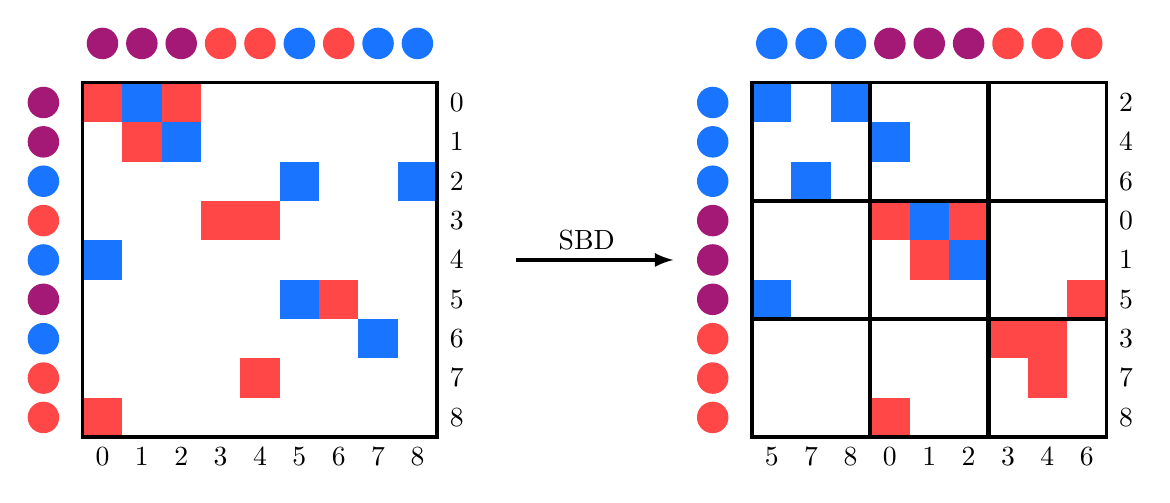
\begin{tikzpicture}[scale=0.5]
		\tikzstyle{myred}=[red!90,opacity=.8]
		\tikzstyle{myblue}=[blue!60!cyan,opacity=.9]
		\tikzstyle{mypurple}=[purple!80!blue,opacity=.9]
		\tikzstyle{myarrow}=[line width=1.3pt,>=latex,->]

		\foreach \x / \y in {1/1,1/3,2/2,4/5,4/4,8/5,6/7,9/1} { \fill[myred] ({\y-1},{-\x+1}) rectangle +(1,-1);}
		\foreach \x / \y in {1/2,2/3,3/6,3/9,6/6,5/1,7/8} { \fill[myblue] ({\y-1},{-\x+1}) rectangle +(1,-1);}
%		\draw[help lines] (0,-9) grid (9,0);
		\foreach \x in {0,1,...,8} {\node at ({9.5},{-\x-.5}) {\x};}
		\foreach \x in {0,1,...,8} {\node at ({\x+.5},-9.5) {\x};}


		\foreach \x in {1,2,3} { \fill[mypurple] ({\x-0.5},1) circle (0.4cm);}
		\foreach \x in {4,5,7} { \fill[myred] ({\x-0.5},1) circle (0.4cm);}
		\foreach \x in {6,8,9} { \fill[myblue] ({\x-0.5},1) circle (0.4cm);}

		\foreach \x in {1,2,6} { \fill[mypurple] (-1,{-\x+0.5}) circle (0.4cm);}
		\foreach \x in {4,8,9} { \fill[myred] (-1,{-\x+0.5}) circle (0.4cm);}
		\foreach \x in {3,5,7} { \fill[myblue] (-1,{-\x+0.5}) circle (0.4cm);}

		\draw[very thick] (0,-9) rectangle (9,0);

		\draw[thick,myarrow] (11,-4.5) -- (15,-4.5);
		\node at (12.8,-4) {SBD};
		\foreach \x / \y in {4/4,4/6,5/5,7/8,7/7,8/8,6/9,9/4} { \fill[myred] ({17+\y-1},{-\x+1}) rectangle +(1,-1);}
		\foreach \x / \y in {1/1,1/3,2/4,3/2,4/5,5/6,6/1} { \fill[myblue] ({17+\y-1},{-\x+1}) rectangle +(1,-1);}

%		\draw[help lines] (17,-9) grid ({17+9},0);
		\foreach \x / \y in {2/0,4/1,6/2,0/3,1/4,5/5,3/6,7/7,8/8} {\node at ({17+9.5},{-\y-.5}) {\x};}
		\foreach \x / \y in {5/0,7/1,8/2,0/3,1/4,2/5,3/6,4/7,6/8} {\node at ({17+\y+.5},-9.5) {\x};}


		\foreach \x in {4,5,6} { \fill[mypurple] ({17+\x-0.5},1) circle (0.4cm);}
		\foreach \x in {7,8,9} { \fill[myred] ({17+\x-0.5},1) circle (0.4cm);}
		\foreach \x in {1,2,3} { \fill[myblue] ({17+\x-0.5},1) circle (0.4cm);}

		\foreach \x in {4,5,6} { \fill[mypurple] ({17-1},{-\x+0.5}) circle (0.4cm);}
		\foreach \x in {7,8,9} { \fill[myred] ({17-1},{-\x+0.5}) circle (0.4cm);}
		\foreach \x in {1,2,3} { \fill[myblue] ({17-1},{-\x+0.5}) circle (0.4cm);}

		\draw[very thick] ({17+0},-9) rectangle ({17+9},0);

		\draw[ultra thick] ({17+3},0) -- ({17+3},-9);
		\draw[ultra thick] ({17+6},0) -- ({17+6},-9);

		\draw[ultra thick] ({17+0},-3) -- ({17+9},-3);
		\draw[ultra thick] ({17+0},-6) -- ({17+9},-6);
	\end{tikzpicture}
	\caption{Example of SBD form of a partitioned matrix. On the left the original matrix is shown whereas on the right we have the permuted SBD form. On the top/left sides of the matrices it is shown whether that row is completely red or blue or it is mixed (purple), whereas on the bottom/right sides the indices of the columns/rows are explicitly given.} \label{fig:sbd}
\end{figure}

More explicitly, if we denote as $m_i := |R_i|$, $n_i := |C_i|$, with $i=0,1,2$, we have that the SBD form is the resulting block matrix:

\begin{align}\dot{A} := A(I,J) = 
	\begin{bmatrix}
		\dot{A}_{00} & \dot{A}_{01}  & \\
		\dot{A}_{10} & \dot{A}_{11} & \dot{A}_{12} \\
		& \dot{A}_{21} & \dot{A}_{22} \\ 
	\end{bmatrix}, \label{eq:sbd}
\end{align}

where

\begin{itemize}
	\item $\dot{A}_{00}$ of size $m_0 \times n_0$, has nonzeros with uncut rows and uncut columns for processor 0;
	\item $\dot{A}_{22}$ of size $m_2 \times n_2$, has nonzeros with uncut rows and uncut columns for processor 1;
	\item $\dot{A}_{01}$ of size $m_0 \times n_1$, has nonzeros with uncut rows for processor 0 and cut columns;
	\item $\dot{A}_{21}$ of size $m_2 \times n_1$, has nonzeros with uncut rows for processor 1 and cut columns;
	\item $\dot{A}_{10}$ of size $m_1 \times n_0$, has nonzeros with cut rows and uncut columns for processor 0;
	\item $\dot{A}_{12}$ of size $m_1 \times n_2$, has nonzeros with cut rows and uncut columns for processor 1;
	\item $\dot{A}_{11}$ of size $m_1 \times n_1$, has nonzeros with cut rows and columns.
\end{itemize}

Note that $m_i$ and $n_i$ can be extremely different, also from matrix to matrix, along with the amount of nonzeros in each block: for example, if the sparsity pattern of the matrix allows a ``perfect'' partitioning such that there is no communication, all blocks are empty except of $\dot{A}_{00}$ and $\dot{A}_{22}$; conversely, if the matrix has a very dense (or complicated) pattern and/or the partitioning is far from the optimal, we might have such blocks almost empty and the central block $\dot{A}_{11}$ with the majority of nonzeros. An example of this difference is shown in Figure \ref{fig:sbd-2}.

\begin{figure}[h]
	\centering
	\subfigure[\texttt{impcol\_b}]{ \includegraphics[scale=0.4]{img/impcol_b.pdf} \label{fig:impcol_b}} \hspace{1cm}
	\subfigure[\texttt{cage7}]{ \includegraphics[scale=0.4]{img/cage6.pdf} \label{fig:cage6} }
	\caption{Example of SBD forms of partitioning of the matrices \texttt{impcol\_b} and \texttt{cage6}. Each part of $\dot{A}$ has been colored differently. In the first matrix there are no cut rows, and therefore $\dot{A}_{10}=\dot{A}_{11} =\dot{A}_{12} = \varnothing$. The images were produced with MATLAB.} \label{fig:sbd-2}
\end{figure}


By computing the Separated Block Diagonal form of a matrix, we are able to explicitly see an underlying structure of the matrix, and the properties of each block can be used to adapt the assignment of its nonzeros. More in particular, the blocks $\dot{A}_{00}$ and $\dot{A}_{22}$ have nonzeros with uncut rows and columns and therefore we ideally want to keep some of the information that these nonzeros fit conveniently together; of course, we still have to assign them to $A_r$ and $A_c$ and, as mentioned earlier, we can't do both, and a convenient thing is to base our choice on the sizes of such blocks. For example, if $m_0 < n_0$, in the block $\dot{A}_{00}$ we have that the columns are (on average) longer than the rows: therefore if we assign the nonzeros of this block to $A_c$ we are, on principle, getting away with more.

For the block with uncut rows ($\dot{A}_{01}$, $\dot{A}_{21}$) and cut columns, the choice is easy: we assign them to $A_r$ and keep their rows uncut. Similarly, we assign the nonzeros of $\dot{A}_{10}$ and $\dot{A}_{12}$ to $A_c$, keeping their column uncut. 

For the middle block $\dot{A}_{11}$, whose nonzeros have cut rows and cut columns, we can't exploit any underlying structure: a possible way is to employ one of the other heuristics described in this chapter only considering this submatrix. Our choice is to go with Algorithm \ref{alg:localview-po} presented in Section \ref{sec:localview} (note that we cannot exploit the partition-aware variant of this algorithm because all of the nonzeros have cut rows and columns).

The heuristic that employs the SBD structure of a matrix is described in Algorithm \ref{alg:sbdview}.

\begin{algorithm}[h]
	\begin{algorithmic}
		\Require{partitioned matrix $A$}
		\Ensure{$A_r$, $A_c$}
		\State
		\State $\dot{A}:=$ SBD form of the partitioned matrix $A$.
		\State $m_0 := |\{ i : \text{ row } i \text{ is fully assigned to processor 0 } \}|$
		\State $m_2 := |\{ i : \text{ row } i \text{ is fully assigned to processor 1 } \}|$
		\State $n_0 := |\{ j : \text{ column } j \text{ is fully assigned to processor 0 } \}|$
		\State $n_2 := |\{ j : \text{ column } j \text{ is fully assigned to processor 1 } \}|$
		\State
		\If{$m_0 < n_0$}
		\State Assign nonzeros of $\dot{A}_{00}$ to $A_r$
		\Else
		\State Assign nonzeros of $\dot{A}_{00}$ to $A_c$
		\EndIf
		\If{$m_2 < n_2$}
		\State Assign nonzeros of $\dot{A}_{22}$ to $A_r$
		\Else
		\State Assign nonzeros of $\dot{A}_{22}$ to $A_c$
		\EndIf
		\State
		\State Assign nonzeros of $\dot{A}_{10}$ to $A_c$
		\State Assign nonzeros of $\dot{A}_{12}$ to $A_c$
		\State Assign nonzeros of $\dot{A}_{01}$ to $A_r$
		\State Assign nonzeros of $\dot{A}_{21}$ to $A_r$
	\end{algorithmic}
	\caption{Assignment of the nonzeros based on the SBD form of the partitioned matrix $A$.} \label{alg:sbdview}
\end{algorithm}

Note that, as mentioned in Chapter \ref{chap:introduction}, the matrix is usually split by means of recursive bipartitionings: it is then sufficient to keep track of the order of these recursions to have an implicit ordering which can be easily used to compute the SBD form of a matrix \cite{yzelman_cache}.

\subsection{Using the Separated Block Diagonal form of order 2 of $A$}

The SBD2 form of a partitioned matrix $A$ is an extension of the SBD form: given a partitioned matrix $A$, we compute the Separate Block Diagonal form of $A$ of order 2 as shown in Algorithm \ref{alg:sbd2}. 

\begin{algorithm}[h]
	\begin{algorithmic}
		\Require{ partitioned matrix $A$}
		\Ensure{$\ddot{A}$}
		\State compute $\dot{A}$ as the SBD form of $A$ and obtain also $R_0,R_1,R_2,C_0,C_1,C_2$;
		\State split $R_0$ in $R_{00}$ and $R_{01}$, such that $A(R_{00},C_1) = \varnothing$;
		\State split $R_2$ in $R_{20}$ and $R_{21}$, such that $A(R_{21},C_1) = \varnothing$;
		\State split $C_0$ in $C_{00}$ and $C_{01}$, such that $A(R_1,C_{00}) = \varnothing$;
		\State split $C_2$ in $C_{20}$ and $C_{21}$, such that $A(R_1,C_{21}) = \varnothing$;
		\State $I:= (R_{00},R_{01},R_1,R_{20},R_{21})$;
		\State $J:= (C_{00},C_{01},C_1,C_{20},C_{21})$;
		\State $\ddot{A} := A(I,J)$.
	\end{algorithmic}
	\caption{Algorithm to obtain SBD2 form of a matrix $A$.} \label{alg:sbd2}
\end{algorithm}

The main idea of this form is to compute a matrix with even more structure, as $\ddot{A}$ is a tridiagonal matrix with $ 5 \times 5$ blocks.

\begin{figure}[h]
	\centering
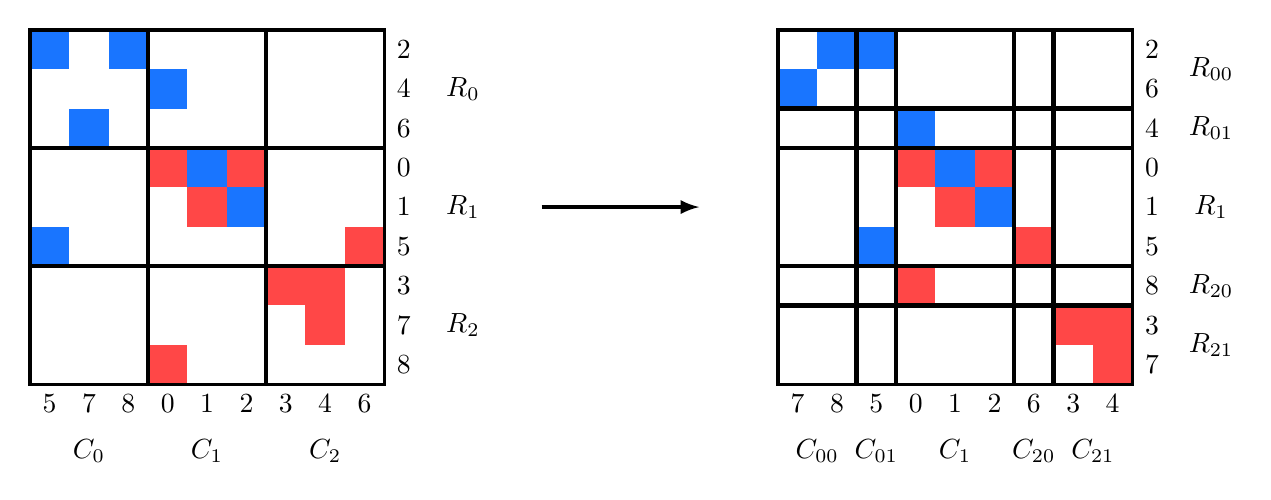
\begin{tikzpicture}[scale=0.5]
	\tikzstyle{myred}=[red!90,opacity=.8]
	\tikzstyle{myblue}=[blue!60!cyan,opacity=.9]
	\tikzstyle{mypurple}=[purple!80!blue,opacity=.9]
	\tikzstyle{myarrow}=[line width=1.3pt,>=latex,->]
			\foreach \x / \y in {4/4,4/6,5/5,7/8,7/7,8/8,6/9,9/4} { \fill[myred] ({0+\y-1},{-\x+1}) rectangle +(1,-1);}
		\foreach \x / \y in {1/1,1/3,2/4,3/2,4/5,5/6,6/1} { \fill[myblue] ({0+\y-1},{-\x+1}) rectangle +(1,-1);}

%		\draw[help lines] (0,-9) grid ({0+9},0);
		\foreach \x / \y in {2/0,4/1,6/2,0/3,1/4,5/5,3/6,7/7,8/8} {\node at ({0+9.5},{-\y-.5}) {\x};}
		\foreach \x / \y in {5/0,7/1,8/2,0/3,1/4,2/5,3/6,4/7,6/8} {\node at ({0+\y+.5},-9.5) {\x};}

		\node at (1.5,-10.7) {$C_0$};
		\node at (4.5,-10.7) {$C_1$};
		\node at (7.5,-10.7) {$C_2$};

		\node at (11,-1.5) {$R_0$};
		\node at (11,-4.5) {$R_1$};
		\node at (11,-7.5) {$R_2$};
		
		\draw[very thick] ({0+0},-9) rectangle ({0+9},0);

		\draw[ultra thick] ({0+3},0) -- ({0+3},-9);
		\draw[ultra thick] ({0+6},0) -- ({0+6},-9);

		\draw[ultra thick] ({0+0},-3) -- ({0+9},-3);
		\draw[ultra thick] ({0+0},-6) -- ({0+9},-6);

		\draw[thick,myarrow] (13,-4.5) -- (17,-4.5);

		\foreach \x / \y in {4/4,4/6,5/5,8/9,8/8,9/9,6/7,7/4} { \fill[myred] ({19+\y-1},{-\x+1}) rectangle +(1,-1);}
		\foreach \x / \y in {1/3,1/2,3/4,2/1,4/5,5/6,6/3} { \fill[myblue] ({19+\y-1},{-\x+1}) rectangle +(1,-1);}

%		\draw[help lines] (19,-9) grid ({19+9},0);
		\foreach \x / \y in {2/0,6/1,4/2,0/3,1/4,5/5,8/6,3/7,7/8} {\node at ({19+9.5},{-\y-.5}) {\x};}
		\foreach \x / \y in {7/0,8/1,5/2,0/3,1/4,2/5,6/6,3/7,4/8} {\node at ({19+\y+.5},-9.5) {\x};}
	
		\node at ({19+1},-10.7) {$C_{00}$};
		\node at ({19+2.5},-10.7) {$C_{01}$};
		\node at ({19+4.5},-10.7) {$C_{1}$};
		\node at ({19+6.5},-10.7) {$C_{20}$};
		\node at ({19+8},-10.7) {$C_{21}$};

		\node at ({19+11},-1) {$R_{00}$};
		\node at ({19+11},-2.5) {$R_{01}$};
		\node at ({19+11},-4.5) {$R_{1}$};
		\node at ({19+11},-6.5) {$R_{20}$};
		\node at ({19+11},-8) {$R_{21}$};
		
		\draw[very thick] ({19+0},-9) rectangle ({19+9},0);

		\draw[ultra thick] ({19+3},0) -- ({19+3},-9);
		\draw[ultra thick] ({19+6},0) -- ({19+6},-9);
		\draw[ultra thick] ({19+2},0) -- ({19+2},-9);
		\draw[ultra thick] ({19+7},0) -- ({19+7},-9);

		\draw[ultra thick] ({19+0},-3) -- ({19+9},-3);
		\draw[ultra thick] ({19+0},-6) -- ({19+9},-6);
		\draw[ultra thick] ({19+0},-2) -- ({19+9},-2);
		\draw[ultra thick] ({19+0},-7) -- ({19+9},-7);
	\end{tikzpicture}
	\caption{SBD2 form obtained starting from the SBD form of Figure \ref{fig:sbd}.}
\end{figure}



\section{Maximizing empty rows of $B$} \label{sec:globalview}

At the beginning of this chapter we mentioned how it is convenient to have full rows assigned to $A_r$ and full columns assigned to $A_c$, in order to avoid communication; a good strategy to produce good $A_r$ and $A_c$ could then be to maximize such full assignments.

The proposed heuristic does substantially this: instead of a generating scheme, it is more of an improvement scheme and, given $A_r$ and $A_c$, it tries to move around nonzeros in order to obtain full rows assigned to $A_r$ and full columns to $A_c$, by considering nonzeros that belong to rows and columns that are both cut. If we change the assignment of those nonzeros, we are sure to not increase the communication volume, while there is still the possibility of decreasing it. 

To have a unique formulation that can obtain full rows assigned to $A_r$ and full columns to $A_c$, it is convenient to reason in terms of the resulting matrix $B$, obtained following the medium-grain model. If we maximize the number of empty rows of $B$, we are effectively emptying rows of $A_r^T$ (which means emptying columns of $A_r$) and of $A_c$. 

\section{Partial assignment of rows and columns} \label{sec:hot_restart}
